\documentclass[varwidth=true, border=2pt]{standalone}

\usepackage{pgfplots}
\usepackage{tikz}
\usetikzlibrary{calc,fadings,decorations.pathreplacing}

\begin{document}
%% helper macros
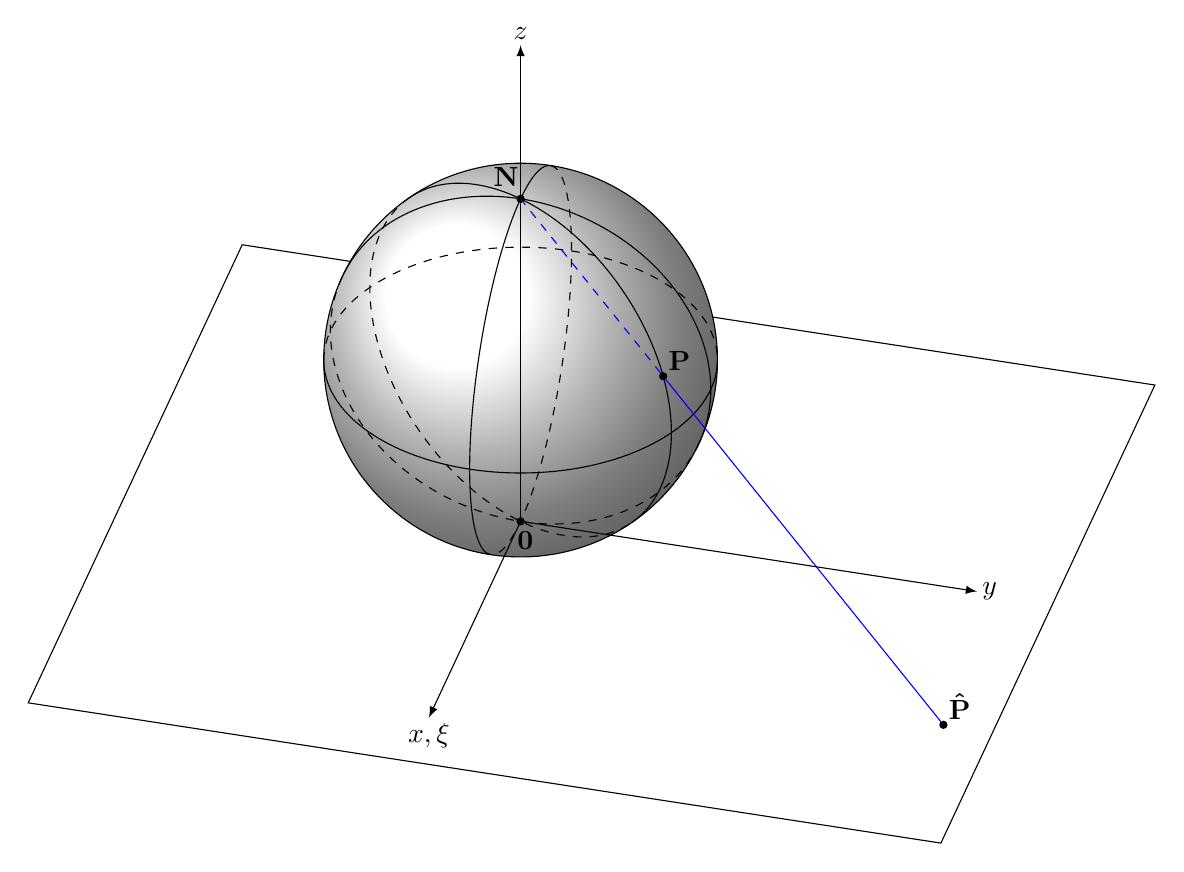
\begin{tikzpicture} % CENT
    \newcommand\pgfmathsinandcos[3]{%
        \pgfmathsetmacro#1{sin(#3)}%
        \pgfmathsetmacro#2{cos(#3)}%
    }
    \newcommand\LongitudePlane[3][current plane]{%
        \pgfmathsinandcos\sinEl\cosEl{#2} % elevation
        \pgfmathsinandcos\sint\cost{#3} % azimuth
        \tikzset{#1/.estyle={cm={\cost,\sint*\sinEl,0,\cosEl,(0,0)}}}
    }
    \newcommand\LatitudePlane[3][current plane]{%
        \pgfmathsinandcos\sinEl\cosEl{#2} % elevation
        \pgfmathsinandcos\sint\cost{#3} % latitude
        \pgfmathsetmacro\yshift{\cosEl*\sint}
        \tikzset{#1/.estyle={cm={\cost,0,0,\cost*\sinEl,(0,\yshift)}}} %
    }
    \newcommand\DrawLongitudeCircle[2][1]{
        \LongitudePlane{\angEl}{#2}
        \tikzset{current plane/.prefix style={scale=#1}}
        % angle of "visibility"
        \pgfmathsetmacro\angVis{atan(sin(#2)*cos(\angEl)/sin(\angEl))} %
        \draw[current plane] (\angVis:1) arc (\angVis:\angVis+180:1);
        \draw[current plane,dashed] (\angVis-180:1) arc (\angVis-180:\angVis:1);
    }
    \newcommand\DrawLatitudeCircle[2][1]{
        \LatitudePlane{\angEl}{#2}
        \tikzset{current plane/.prefix style={scale=#1}}
        \pgfmathsetmacro\sinVis{sin(#2)/cos(#2)*sin(\angEl)/cos(\angEl)}
        % angle of "visibility"
        \pgfmathsetmacro\angVis{asin(min(1,max(\sinVis,-1)))}
        \draw[current plane] (\angVis:1) arc (\angVis:-\angVis-180:1);
        \draw[current plane,dashed] (180-\angVis:1) arc (180-\angVis:\angVis:1);
    }

    \tikzset{%
        >=latex, % option for nice arrows
        inner sep=0pt,%
        outer sep=2pt,%
        mark coordinate/.style={inner sep=0pt,outer sep=0pt,minimum size=3pt,
                fill=black,circle}%
    }
    %% some definitions

    \def\R{2.5} % sphere radius
    \def\angEl{35} % elevation angle
    \def\angAz{-105} % azimuth angle
    \def\angPhi{-40} % longitude of point P
    \def\angBeta{19} % latitude of point P

    %% working planes

    \pgfmathsetmacro\H{\R*cos(\angEl)} % distance to north pole
    \tikzset{xyplane/.estyle={cm={cos(\angAz),sin(\angAz)*sin(\angEl),-sin(\angAz),
                        cos(\angAz)*sin(\angEl),(0,-\H)}}}
    \LongitudePlane[xzplane]{\angEl}{\angAz}
    \LongitudePlane[pzplane]{\angEl}{\angPhi}
    \LatitudePlane[equator]{\angEl}{0}

    %% draw xyplane and sphere

    \draw[xyplane] (-2*\R,-2*\R) rectangle (2.2*\R,2.8*\R);
    \fill[ball color=white] (0,0) circle (\R); % 3D lighting effect
    \draw (0,0) circle (\R);

    %% characteristic points

    \coordinate (O) at (0,0);
    \coordinate[mark coordinate] (N) at (0,\H);
    \coordinate[mark coordinate] (S) at (0,-\H);
    \path[pzplane] (\angBeta:\R) coordinate[mark coordinate] (P);
    \path[pzplane] (\R,0) coordinate (PE);
    \path[xzplane] (\R,0) coordinate (XE);
    \path (PE) ++(0,-\H) coordinate (Paux); % to aid Phat calculation
    \coordinate[mark coordinate] (Phat) at (intersection cs: first line={(N)--(P)},
    second line={(S)--(Paux)});

    %% draw meridians and latitude circles

    \DrawLatitudeCircle[\R]{0} % equator
    \DrawLongitudeCircle[\R]{\angAz} % xzplane
    \DrawLongitudeCircle[\R]{\angAz+90} % yzplane
    \DrawLongitudeCircle[\R]{\angPhi} % pzplane

    %% draw xyz coordinate system

    \draw[xyplane,<->] (1.8*\R,0) node[below] {$x,\xi$} -- (0,0) -- (0,2.4*\R)
    node[right] {$y$};
    \draw[->] (0,-\H) -- (0,1.6*\R) node[above] {$z$};

    %% draw lines and put labels

    \draw[blue,dashed] (P) -- (N) +(0.3ex,0.6ex) node[above left,black] {$\mathbf{N}$};
    \draw[blue] (P) -- (Phat) node[above right,black] {$\mathbf{\hat{P}}$};
    \path (S) +(0.4ex,-0.4ex) node[below] {$\mathbf{0}$};
    \draw (P) node[above right] {$\mathbf{P}$};
\end{tikzpicture}

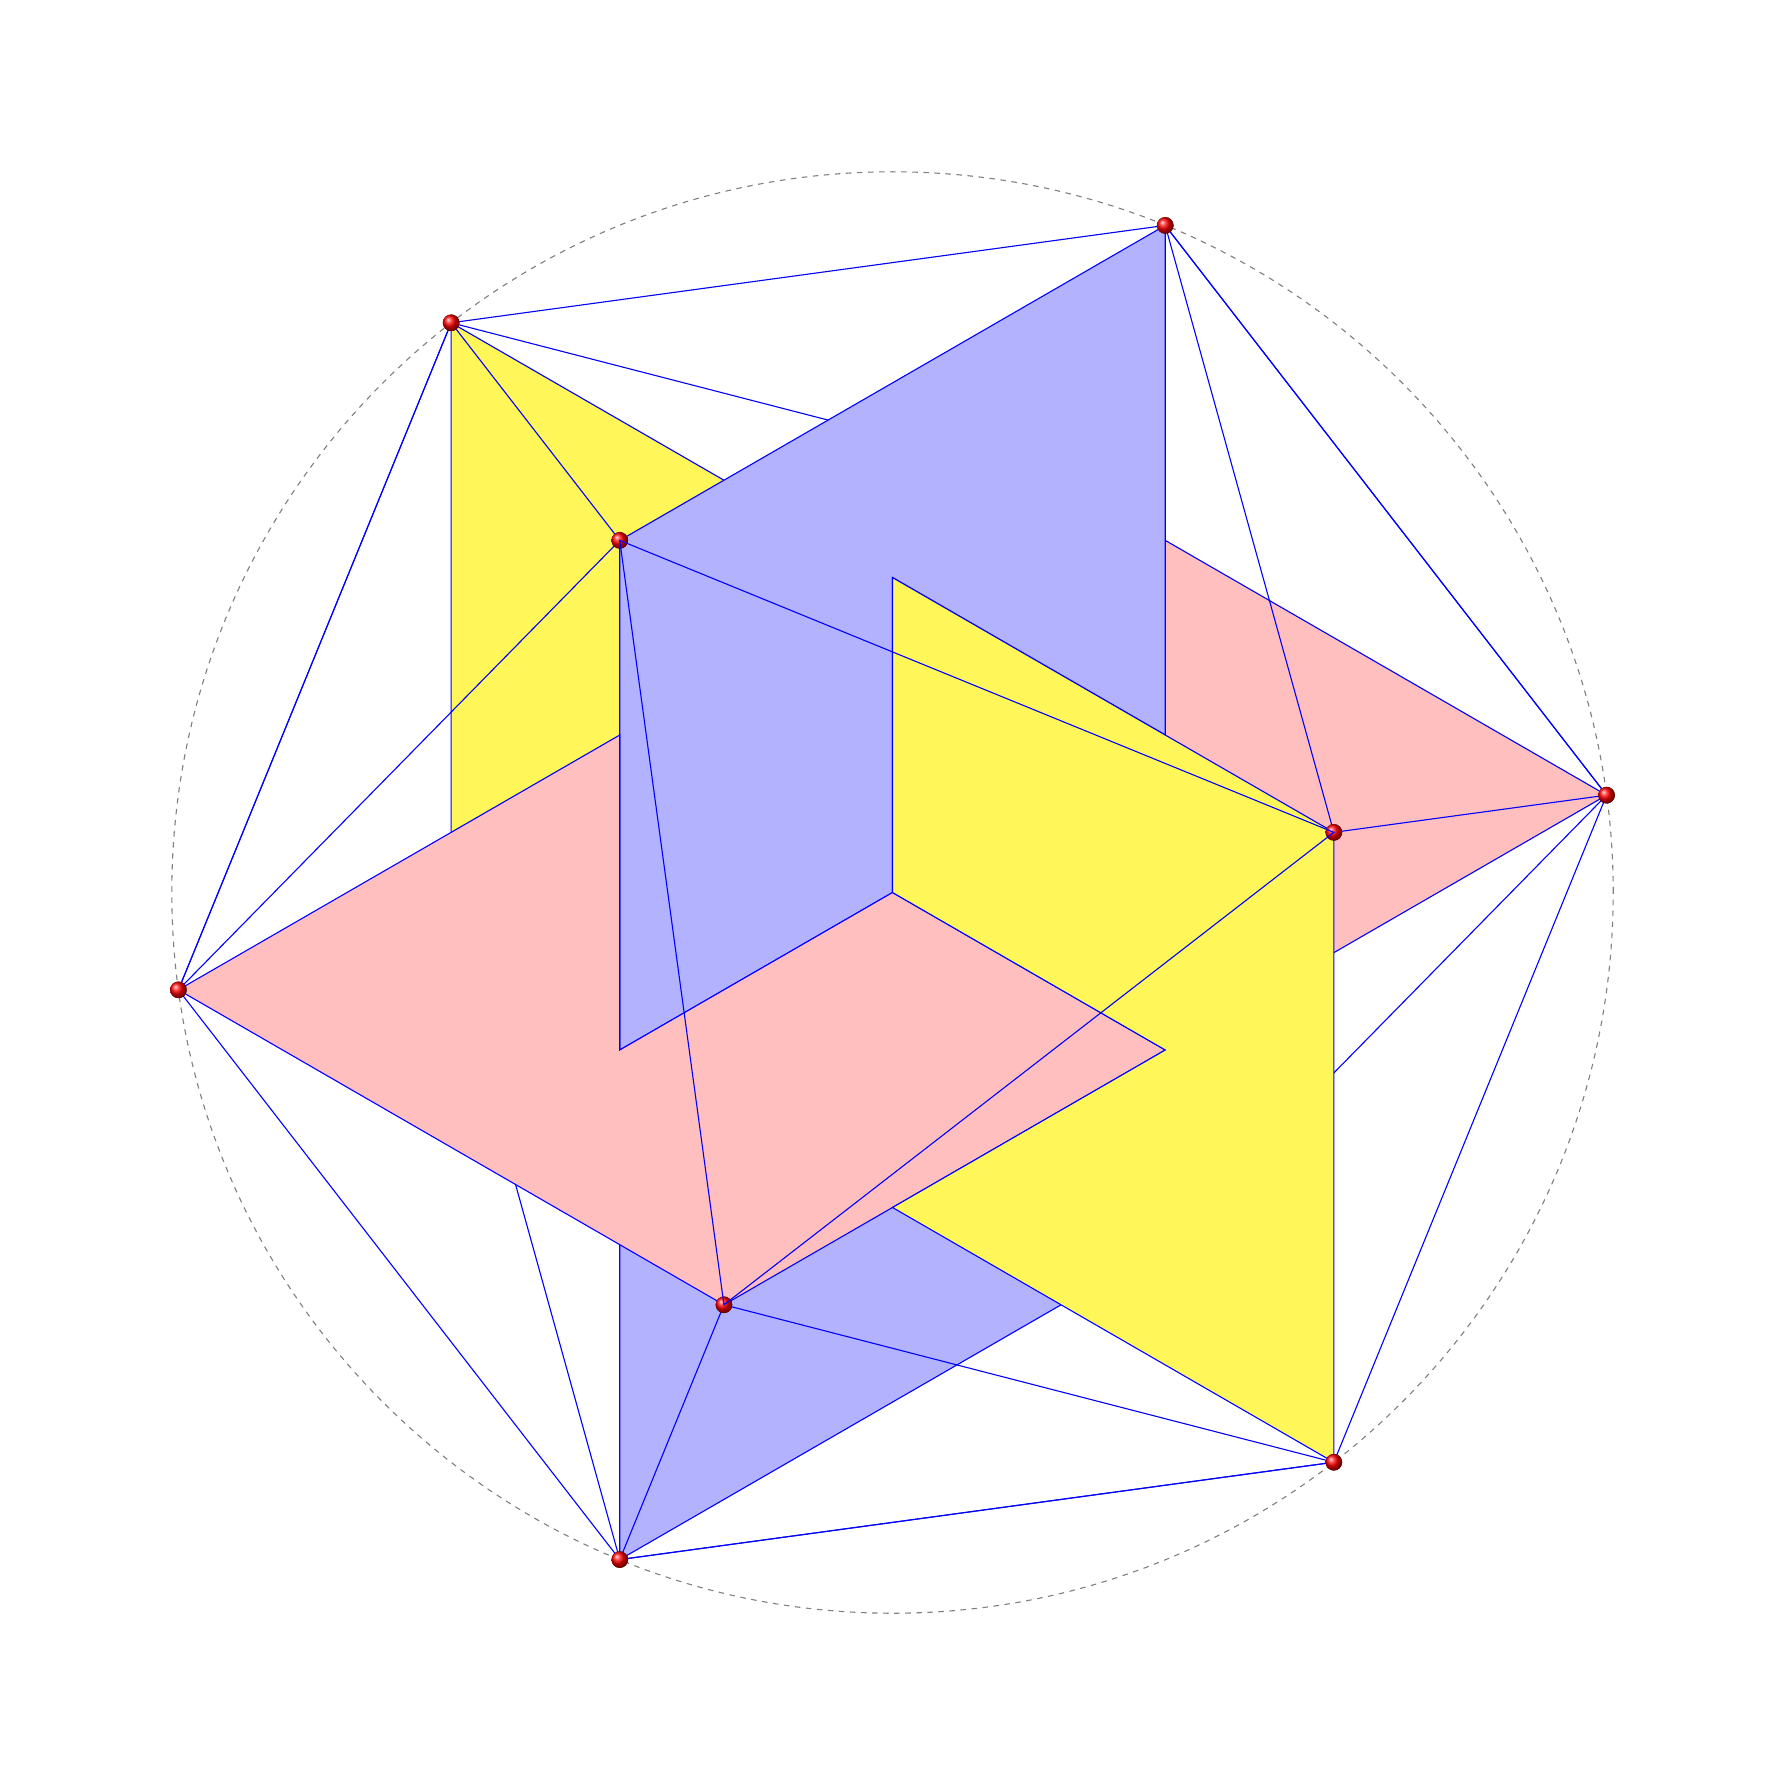
\begin{tikzpicture}
    \def\rm{4}
    \pgfmathsetmacro{\R}{sqrt(1+(1+sqrt(5))^2/4+(1+sqrt(5))/2)*\rm}
    \pgfmathsetmacro{\rh}{sqrt(1+(1+sqrt(5))^2/4-(1+sqrt(5))/2)*\rm};
    \pgfmathsetmacro{\b}{\rm*(1+sqrt(5))/2}
    \pgfmathsetmacro{\goc}{acos(((\rm)^2-(\b)^2+(\R)^2)/(2*(\rm)*(\R)))}
    \clip (0,0) circle(1.2*\R);
    \foreach \i in{0,1,2}{
            \path (90+\i*120:\rm)coordinate(A\i);
            \draw (0,0)--(A\i);
        }
    \foreach \j in{0,1,2}{
            \pgfmathsetmacro{\jh}{\j+1}
            \path (90+\goc+ \j*120:\rh)coordinate(B\j);
        }
    \foreach \k in{0,1,...,5}{
            \pgfmathsetmacro{\kh}{\k+1}
            \draw[blue](90+\goc+60*\k:\R)coordinate(C\k)--(90+\goc+60*\kh:\R);
        }
    \foreach \y/\mau in{0/pink,120/yellow!65,240/blue!30}{
            \draw[blue,rotate=\y](90+\goc:\R)--(90+300+\goc:\rh);
            \draw[blue,rotate=\y,fill=\mau](0,0)--(-30:\rm)--([turn]60:\b)--([turn]120:2*\rm)--(0,0);
            \draw [blue,rotate=\y](90+\goc+240:\rh)--(90+\goc+240:\R)--(390+\goc:\R)--cycle;
        }
    \foreach \n/\mau in{0/blue!30,120/pink,240/yellow!65}{
            \draw[blue,rotate=\n,fill=\mau](90:\rm)--(0,0)--([turn]-60:\rm)--++(90:\b)--([turn]-60:2*\rm)--++(-90:\b)--cycle;
        }
    \draw [dash pattern ={on 2pt off 2pt},gray](0,0)circle(\R cm);
    \foreach \x in{0,1,2}{
            \fill[ball color=red](B\x)circle(3pt);}
    \draw[blue](B0)--(B2)--(B1)--cycle;
    \foreach \x in{0,1,...,5}{
            \fill[ball color=red](C\x)circle(3pt);}
\end{tikzpicture}
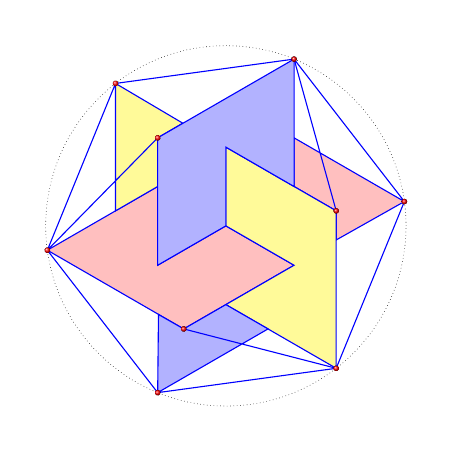
\begin{tikzpicture}
    \def\r{1} \pgfmathsetmacro\b{\r*(1+sqrt(5))/2}
    \pgfmathsetmacro\a{sqrt(1+(1+sqrt(5))^2/4-(1+sqrt(5))/2)*\r}
    \pgfmathsetmacro\R{sqrt(1+(1+sqrt(5))^2/4+(1+sqrt(5))/2)*\r}
    \pgfmathsetmacro\g{acos(((\r)^2-(\b)^2+(\R)^2)/(2*(\r)*(\R)))}
    \clip (0,0) circle(\R*1.1);
    \draw[densely dotted,very thin] (0,0) circle(\R);
    \foreach \i/\mau in {0/pink,1/yellow!40,2/blue!30}{
            \fill[rotate=\i*120,\mau] (0,0)--(-30:\r)--(-150+\g:\a)--(-210+\g:\R)--(150:\r)--(210:\r)--cycle (-30+\g:\R)--(-45+\g:\a)--(-30+\g:\a)--(30:\r)--(14.5+\g:\a)--cycle;% tô màu
            \draw[rotate=\i*120,blue] % vẽ đường màu xanh
            (0,0)--(-30:\r)--(-150+\g:\a)--(-210+\g:\R)--(150:\r)--(210:\r)--cycle (-30+\g:\R)--(-45+\g:\a)--(-30+\g:\a)--(30:\r)--(14.5+\g:\a)--cycle
            (-90+\g:\R)--(-30+\g:\R)--(30+\g:\R)--(-30+\g:\a);}
    \foreach \i in{0,1,2}{
            \fill[rotate=\i*120,ball color=red](-30+\g:\a)circle(1pt);
            \fill[rotate=\i*120,ball color=red](-30+\g:\R)circle(1pt);
            \fill[rotate=\i*120,ball color=red](30+\g:\R)circle(1pt);}
\end{tikzpicture}
\end{document}